\documentclass[preprint,12pt]{elsarticle}

% -----------------------------------------------------
% Core packages
% -----------------------------------------------------
\usepackage[utf8]{inputenc}
\usepackage[T1]{fontenc}
\usepackage{graphicx}
\usepackage{amsmath}
\usepackage{amssymb}
\usepackage{booktabs}
\usepackage{array}
\usepackage{tabularx}
\usepackage{multirow}
\usepackage{placeins}
\usepackage{float}
\usepackage{algorithm}
\usepackage{algpseudocode}
\usepackage[table]{xcolor}
\usepackage{tikz}
\usetikzlibrary{positioning,calc}
\usepackage[protrusion=true,expansion=false]{microtype}
\usepackage{url}
\usepackage{setspace}
\onehalfspacing

\algrenewcommand\algorithmicrequire{\textbf{Input:}}
\algrenewcommand\algorithmicensure{\textbf{Output:}}

% -----------------------------------------------------
% Global visual semantics
% Color encodes result direction, not model identity.
% -----------------------------------------------------
\definecolor{Positive}{HTML}{3F8C7A} % positive/supportive direction
\definecolor{Negative}{HTML}{B05A4F} % negative/adverse direction
\definecolor{Neutral}{HTML}{7A838A}  % structure/control/baseline
\definecolor{Ink}{HTML}{454B50}      % borders/arrows/text accents

\colorlet{PositiveCell}{Positive!14}
\colorlet{NegativeCell}{Negative!14}
\colorlet{NeutralCell}{Neutral!10}

\newcommand{\poscell}[1]{\cellcolor{PositiveCell}#1}
\newcommand{\negcell}[1]{\cellcolor{NegativeCell}#1}
\newcommand{\neutralcell}[1]{\cellcolor{NeutralCell}#1}

% -----------------------------------------------------
% Clickable references and PDF outline/bookmarks
% -----------------------------------------------------
\usepackage[
    unicode=true,
    colorlinks=true,
    linkcolor=blue,
    citecolor=blue,
    urlcolor=black,
    bookmarks=true,
    bookmarksopen=true,
    bookmarksnumbered=true,
    bookmarksopenlevel=2,
    pdfpagemode=UseOutlines,
    pdftitle={Rule-Constrained Fine-Tuning and Task Transfer in Large Language Models: Behavioral Evaluation and Causal Analysis of Attention Heads},
    pdfsubject={Rule-constrained fine-tuning, task transfer, and causal attention-head analysis},
    pdfkeywords={rule-constrained fine-tuning, task transfer, constraint-sensitive decision making, mechanistic interpretability, attention-head ablation}
]{hyperref}
\usepackage{bookmark}
\bookmarksetup{open,numbered}

\def\urlprefix{URL:\nobreak\hspace{0.25em}}

\biboptions{sort&compress}

\newcommand{\figref}[1]{Fig.~\ref{#1}}
\newcommand{\tabref}[1]{Table~\ref{#1}}
\newcommand{\secref}[1]{Section~\ref{#1}}
\newcommand{\equref}[1]{Eq.~\ref{#1}}

% Remove the default title-page preprint footer, following the supplied
% Neurocomputing reference project.
\makeatletter
\def\ps@pprintTitle{%
  \let\@oddhead\@empty
  \let\@evenhead\@empty
  \let\@oddfoot\@empty
  \let\@evenfoot\@empty
}
\makeatother

\begin{document}

\begin{frontmatter}

\title{Rule-Constrained Fine-Tuning and Task Transfer in Large Language Models:
Behavioral Evaluation and Causal Analysis of Attention Heads}

% Fill the final author/affiliation information before submission.
% \author[aff1]{First Author}
% \author[aff1]{Second Author\corref{cor1}}
% \cortext[cor1]{Corresponding author\\ Email: example@university.edu}
% \address[aff1]{Department, University, City, Country}

\begin{abstract}

Fine-tuning can reshape model behavior beyond the source task, but it remains unclear whether structured decision training transfers reusable operations across tasks and how explicit constraints alter this transfer. We investigate these questions using Dou Dizhu, a rule-rich decision environment, and compare ordinary task adaptation with rule-constrained fine-tuning across three open-weight language model checkpoints. Cross-task evaluation shows that ordinary fine-tuning produces strongly model-dependent transfer, whereas constraint-enriched supervision yields a more consistently positive improvement over ordinary adaptation, while remaining selective across reasoning categories. Controlled decision probes further show that rule-constrained adaptation strengthens constraint-induced relative preference shifts, although this probability-level change does not translate into improved greedy-decoding compliance. Causal attention-head ablation on Qwen2.5-7B reveals sparse and heterogeneous changes in functional dependence, with a small subset of heads contributing disproportionately to the measured preference shift. Overall, the results suggest that structured fine-tuning induces selective behavioral transfer and localized mechanistic reorganization rather than a uniform improvement in reasoning ability.

\end{abstract}


\begin{keyword}
Rule-constrained fine-tuning
\sep Task transfer
\sep Constraint-sensitive decision making
\sep Mechanistic interpretability
\sep Attention-head ablation
\end{keyword}

\end{frontmatter}

\section{Introduction}
\label{sec:introduction}

Fine-tuning adapts pretrained language models to downstream tasks and domains through task-specific supervision, while parameter-efficient methods such as Low-Rank Adaptation (LoRA) make this adaptation possible with only a small number of trainable parameters \cite{hu2022lora}. Instruction tuning further shows that supervised adaptation across collections of tasks can improve generalization to unseen tasks \cite{wei2022finetuned,chung2024scaling}. However, an important question remains unclear: when a model learns a structured decision policy through fine-tuning, do the resulting changes represent transferable decision operations, constraint-sensitive behavioral adaptation, or merely surface-level improvements specific to the training domain?

This question is particularly important for decision tasks in which the preferred action depends on changing conditions. In realistic scenarios, effective decision making requires more than mapping an input state to a fixed output. A previously preferred action may become invalid after an additional rule, prohibition, or contextual constraint is introduced, requiring the model to suppress that action and select an alternative. We refer to this setting as \emph{rule-constrained fine-tuning}. Compared with ordinary task fine-tuning, rule-constrained examples explicitly supervise how decisions should change when the admissible action space is modified, providing a controlled environment for studying conditional decision behavior.

A key challenge in studying such transfer is separating task-specific surface forms from underlying decision operations. Improvements on conventional benchmarks may reflect better instruction following, memorized task knowledge, or shared linguistic patterns, rather than transfer of reusable reasoning structures. Therefore, a stricter evaluation should examine whether behaviors learned in one structured domain remain effective when the original terminology and context are replaced by different but structurally related tasks.

To investigate this problem, we use Dou Dizhu as a structured source domain. The choice of Dou Dizhu is not intended to study game playing itself, but to provide a compact environment that combines several properties relevant to controlled decision analysis. Unlike many classical rule-based environments that focus primarily on fixed planning or adversarial search, Dou Dizhu contains hierarchical relations, combinatorial patterns, legal action constraints, and conditional action selection within a unified decision process. These characteristics make it suitable for studying whether fine-tuning can transfer abstract decision operations beyond source-domain surface forms.

We construct a mixed fine-tuning corpus containing 50,400 general instruction examples and 5,500 Dou Dizhu decision examples. The general component is included to reduce over-specialization to the game-specific format, while the Dou Dizhu component supplies repeated structured decision signals. We evaluate two adaptation regimes built around this mixture. We refer to the ordinary condition as Dou Dizhu LoRA (DD-LoRA) and the rule-constrained condition as Rule-Constrained LoRA (RC-LoRA). DD-LoRA uses ordinary Dou Dizhu decision examples, whereas RC-LoRA modifies 851 of the 5,500 Dou Dizhu examples (15.5\%) by adding explicit prohibitions that invalidate an otherwise preferred action and require selection of a legal alternative. This three-way comparison among Base, DD-LoRA, and RC-LoRA separates the transfer associated with ordinary structured-task adaptation from the additional performance changes observed under constraint-enriched supervision.

We study this problem from three complementary perspectives. First, we evaluate whether decision structures learned from the source domain transfer to tasks with different surface forms. To this end, we introduce the Abstracted Cognitive Logic Benchmark (ACL Bench), a 300-item benchmark that abstracts source-domain decision operations into three reasoning categories: Hierarchy Logic, Pattern Recognition, and Counter Logic. ACL Bench removes domain-specific terminology while preserving underlying structural operations, enabling evaluation of whether fine-tuning is associated with transfer at the level of reasoning structure.

Second, we examine how fine-tuning changes model behavior when explicit constraints invalidate previously preferred actions. Rather than measuring only whether a prohibited action becomes less likely, we quantify how an explicit prohibition changes the relative log-probability margin between that action and the strongest legal alternative. We therefore construct controlled constraint-sensitive decision probes and introduce the Best Constraint Delta Margin (BCDM), a log-probability-based metric for measuring constraint-induced relative preference shifts.

Third, behavioral evaluation cannot reveal how the internal components supporting the measured preference shift differ between model states. For Qwen2.5-7B, we therefore perform causal intervention analysis to compare functional dependence across attention heads between Base and RC-LoRA. This analysis characterizes the internal support for the BCDM-based behavior rather than directly explaining the source of cross-task transfer.

\begin{figure}[ht]
\centering
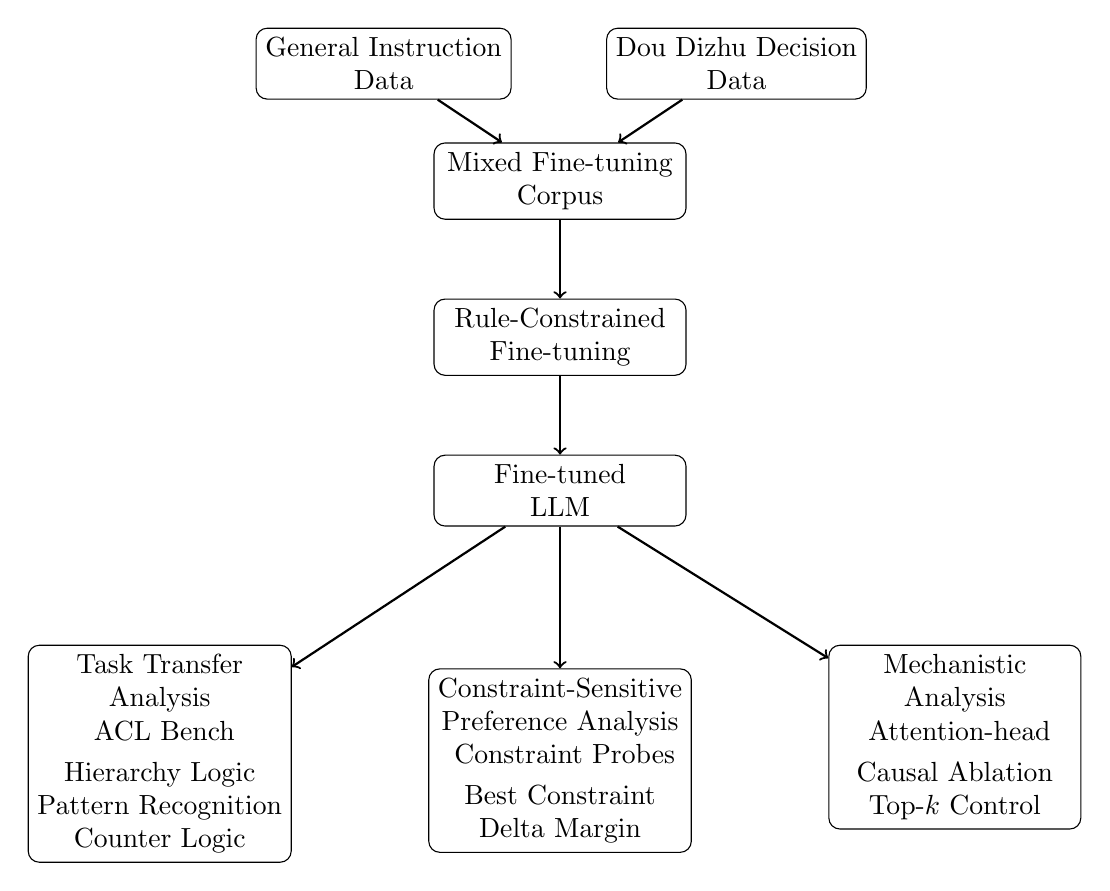
\begin{tikzpicture}[
node distance=1.2cm,
box/.style={
draw,
rounded corners,
align=center,
minimum width=3.2cm,
minimum height=0.8cm
},
smallbox/.style={
draw,
rounded corners,
align=center,
minimum width=2.8cm,
minimum height=0.7cm
},
arrow/.style={
->,
thick
}
]


% Training data

\node (general) [smallbox]
{General Instruction\\Data};

\node (doudizhu) [smallbox, right=1.2cm of general]
{Dou Dizhu Decision\\Data};


\node (corpus) [box, below=1cm of $(general)!0.5!(doudizhu)$]
{Mixed Fine-tuning\\Corpus};


\draw[arrow] (general) -- (corpus);
\draw[arrow] (doudizhu) -- (corpus);


% Fine tuning

\node (finetune) [box, below=1cm of corpus]
{Rule-Constrained\\Fine-tuning};


\draw[arrow] (corpus) -- (finetune);


% Model

\node (model) [box, below=1cm of finetune]
{Fine-tuned\\LLM};


\draw[arrow] (finetune) -- (model);



% Three branches

\node (transfer) [box, below left=1.5cm and 1.8cm of model]
{
Task Transfer\\Analysis\\
\vspace{0.1cm}
ACL Bench\\
Hierarchy Logic\\
Pattern Recognition\\
Counter Logic
};


\node (constraint) [box, below=1.8cm of model]
{
Constraint-Sensitive\\
Preference Analysis\\
\vspace{0.1cm}
Constraint Probes\\
Best Constraint\\
Delta Margin
};


\node (mechanism) [box, below right=1.5cm and 1.8cm of model]
{
Mechanistic\\
Analysis\\
\vspace{0.1cm}
Attention-head\\
Causal Ablation\\
Top-$k$ Control
};


\draw[arrow] (model) -- (transfer);
\draw[arrow] (model) -- (constraint);
\draw[arrow] (model) -- (mechanism);


\end{tikzpicture}
\caption{
Overview of the proposed rule-constrained fine-tuning framework.
The framework integrates structured domain adaptation, cross-task transfer evaluation, constraint-sensitive behavioral analysis, and causal investigation of internal model changes.
}
\label{fig:framework}
\end{figure}


Our experiments reveal three main findings. First, ordinary DD-LoRA already produces selective cross-task transfer, but its effect is highly model-dependent: it improves overall ACL Bench performance for DeepSeek-R1-Distill-Llama-8B and Qwen2.5-7B while slightly reducing performance for Llama3.1-8B. RC-LoRA then yields a positive overall increment relative to DD-LoRA for all three checkpoints, giving a more consistently positive cross-checkpoint transfer profile under the constraint-enriched regime. Second, for Qwen2.5-7B, RC-LoRA exhibits a substantially larger BCDM than Base, indicating a larger constraint-induced relative preference shift; this probability-level change does not translate into improved rule-compliant generation and, under greedy decoding, RC-LoRA selects the prohibited action in all 60 probes. Third, the Base-to-RC-LoRA causal comparison reveals sparse and heterogeneous changes in attention-head contributions, indicating selective changes in functional dependence rather than uniform modification across the attention system.

The main contributions of this work are summarized as follows:

\begin{itemize}

    \item We establish a structured comparison among Base, DD-LoRA, and RC-LoRA, providing an empirical reference for distinguishing ordinary task-transfer effects from the additional changes associated with explicit constraint supervision.

    \item We introduce ACL Bench and BCDM to separately evaluate structural task transfer and constraint-induced relative preference shifts.

    \item We use causal interventions on attention heads to characterize changes in functional dependence associated with constraint-sensitive decision behavior after rule-constrained fine-tuning.

\end{itemize}


The remainder of this paper is organized as follows. Section~\ref{sec:related_work} reviews related work on fine-tuning transfer, constraint following, and mechanistic interpretability. Section~\ref{sec:method} introduces the proposed framework, benchmark construction, and evaluation metrics. Section~\ref{sec:experimental_setup} describes the experimental settings. Section~\ref{sec:results} presents the behavioral and causal analysis results. Section~\ref{sec:discussion} discusses limitations and implications. Finally, Section~\ref{sec:conclusion} concludes the study.

\section{Related Work}
\label{sec:related_work}

\subsection{Fine-Tuning and Cross-Task Generalization}
\label{sec:rw_transfer}

Instruction tuning has shown that supervision on one collection of tasks can improve performance beyond the exact training instances. FLAN demonstrated substantial zero-shot improvements on previously unseen tasks after instruction tuning across heterogeneous datasets \cite{wei2022finetuned}, while T0 showed that multitask prompted training can support generalization to held-out task formulations \cite{sanh2022multitask}. Subsequent work further demonstrated that increasing task diversity, model scale, and reasoning-oriented supervision can improve generalization across broad benchmark collections \cite{chung2024scaling}.

These studies establish that fine-tuning can produce behavioral effects beyond the immediate training data. However, generalization across heterogeneous benchmark collections does not necessarily reveal what has transferred. Improved performance may result from better instruction interpretation, broader task exposure, shared linguistic patterns, or reusable reasoning operations.

Broad benchmarks such as MMLU and BIG-Bench evaluate language models across diverse reasoning and knowledge domains \cite{hendrycks2021measuring,srivastava2022beyond}. Our setting addresses a narrower question. Rather than testing general competence across unrelated tasks, we study whether recurring decision operations learned from a single structured source domain transfer when the original terminology and context are removed. ACL Bench therefore focuses on structurally related transfer through Hierarchy Logic, Pattern Recognition, and Counter Logic.

This distinction also motivates category-level evaluation. Uniform improvement across reasoning categories would be consistent with a broad capability gain, whereas selective changes across structurally different categories provide a more fine-grained view of what fine-tuning transfers. Low-Rank Adaptation (LoRA) makes this question particularly relevant because substantial behavioral adaptation can be achieved without full-model retraining \cite{hu2022lora}.

\subsection{Constraint Following and Rule-Aware Decision Making}
\label{sec:rw_constraints}

Recent work on instruction following has increasingly emphasized explicit constraint satisfaction rather than general response quality. IFEval introduced a reproducible benchmark based on objectively verifiable instructions, including requirements on response length, keywords, and formatting \cite{zhou2023ifeval}. FollowBench extended this direction to multiple categories of fine-grained constraints and progressively more complex combinations of requirements \cite{jiang2024followbench}. These studies show that satisfying explicit constraints constitutes a distinct challenge even for strong language models.

The rule-constrained setting considered in this work differs from conventional response-level constraint evaluation. Rather than specifying properties that the final response must satisfy, our constraints modify the admissible decision space. A previously preferred action can become explicitly prohibited, requiring the model to revise its preference and select a legal alternative.

This distinction motivates our emphasis on preference reallocation. Suppressing the probability of a prohibited action does not necessarily imply that probability has been redirected toward an appropriate alternative. The best constraint delta margin is therefore designed to characterize the relative shift between a forbidden action and the strongest legal alternative. In this respect, our work complements existing constraint-following benchmarks by examining how fine-tuning changes decision preference when the set of admissible actions changes.

\subsection{Mechanistic Interpretability and Fine-Tuning}
\label{sec:rw_mechanistic}

Behavioral evaluation alone cannot determine which internal model components become more or less important after adaptation. Mechanistic interpretability addresses this limitation through causal interventions and circuit-level analyses that identify components functionally involved in specific behaviors \cite{elhage2021mathematical,meng2022locating,conmy2023automated}.

Prior work has shown that individual attention heads can implement behaviorally meaningful computations. Olsson et al.\ identified induction heads associated with sequence-completion behavior and provided causal evidence for their functional role \cite{olsson2022induction}. Intervention-based approaches have also demonstrated that causal perturbations can reveal internal components that are important for particular model outputs or computations \cite{meng2022locating,conmy2023automated}. These findings motivate the use of causal intervention rather than attention magnitude or correlation alone when evaluating functional importance.

More recent studies have examined how fine-tuning changes internal mechanisms. Prakash et al.\ found that fine-tuned models performing entity tracking largely reused mechanisms already present in the base model, with improved performance associated with strengthening of pre-existing circuitry \cite{prakash2024finetuning}. Chhabra et al.\ further reported localized amplification, disruption, and recovery of task-relevant mechanisms under different fine-tuning conditions \cite{chhabra2025neuroplasticity}. Together, these results suggest that fine-tuning can selectively modify the functional importance of existing model components rather than uniformly altering the network.

Our mechanistic analysis follows this intervention-based perspective but focuses on constraint-sensitive decision behavior. We compare attention-head causal contributions before and after fine-tuning and subsequently test whether the heads showing the largest changes form a functionally distinctive subset. Importantly, this analysis concerns the internal support for constraint-sensitive preference adaptation; it does not by itself establish the causal mechanism underlying ACL Bench transfer.

\begin{table}[ht]
\centering
\small
\caption{Comparison between representative related research directions and the present study.}
\label{tab:related_work_comparison}
\begin{tabularx}{\linewidth}{@{}
>{\raggedright\arraybackslash}p{0.18\linewidth}
>{\raggedright\arraybackslash}p{0.27\linewidth}
>{\raggedright\arraybackslash}X@{}}
\toprule
\rowcolor{NeutralCell}
\textbf{Research direction} &
\textbf{Representative work} &
\textbf{Relation to the present study} \\
\midrule

Cross-task generalization &
FLAN \cite{wei2022finetuned}, T0 \cite{sanh2022multitask}, FLAN scaling \cite{chung2024scaling} &
Studies generalization across heterogeneous tasks; our work isolates transfer of structurally related decision operations from a single structured source domain. \\

Constraint following &
IFEval \cite{zhou2023ifeval}, FollowBench \cite{jiang2024followbench} &
Evaluates compliance with directly verifiable response requirements; our setting changes the admissible action space and examines preference reallocation after a preferred action is prohibited. \\

Mechanistic interpretability &
Olsson et al.\ \cite{olsson2022induction}, Meng et al.\ \cite{meng2022locating}, Conmy et al.\ \cite{conmy2023automated} &
Uses causal intervention to identify functionally important components; our work compares attention-head causal contributions before and after rule-constrained fine-tuning. \\

Mechanisms after fine-tuning &
Prakash et al.\ \cite{prakash2024finetuning}, Chhabra et al.\ \cite{chhabra2025neuroplasticity} &
Studies reuse and modification of internal mechanisms after adaptation; our work focuses specifically on causal dependence associated with constraint-sensitive preference changes. \\

\bottomrule
\end{tabularx}
\end{table}

\FloatBarrier

Overall, the present study lies at the intersection of three research directions: cross-task transfer after fine-tuning, explicit constraint-sensitive decision making, and causal analysis of fine-tuned models. The central distinction is that these three levels are evaluated within the same controlled source-domain setting while remaining analytically separate: ACL Bench measures structural task transfer, constraint-sensitive probes measure preference reallocation, and causal intervention examines the internal components supporting the latter behavior.
\section{Method}
\label{sec:method}

Our study investigates rule-constrained fine-tuning from three complementary levels: source-domain training, cross-task behavioral transfer, and internal causal dependence. We first construct a mixed fine-tuning corpus in which a subset of structured decision examples contains explicit prohibitive constraints. We then evaluate cross-task transfer using ACL Bench, a benchmark designed to preserve structural operations from the source domain while changing their surface form. To characterize the learned constraint-sensitive preference reallocation more directly, we construct controlled decision probes and introduce the best constraint delta margin. Finally, we perform complete single-head causal ablation and Top-$k$ joint interventions to examine how fine-tuning changes the functional importance of individual attention heads.

\subsection{Dataset Construction}
\label{sec:dataset_construction}

\subsubsection{Mixed Fine-Tuning Corpus}

We use Dou Dizhu as a structured rule-based decision environment. The purpose of the source domain is not to optimize game-playing performance itself, but to provide repeated examples of hierarchical comparison, structured pattern recognition, legal-action selection, and conditional decision adjustment.

The final fine-tuning corpus contains 55,900 instruction--response examples, consisting of 50,400 general instruction examples and 5,500 Dou Dizhu decision examples. The general instruction data are included to preserve broad instruction-following behavior, while the domain-specific examples expose the model to the structured decision operations of interest.

All fine-tuned models are adapted using Low-Rank Adaptation (LoRA) \cite{hu2022lora}, allowing task-specific behavior to be learned while keeping the pretrained model parameters frozen.

\subsubsection{Ordinary and Rule-Constrained Decision Examples}

We distinguish between ordinary decision examples and rule-constrained decision examples.

An ordinary decision example can be represented as

\[
x \rightarrow a^{*},
\]

where $x$ denotes the current decision state and $a^{*}$ is the preferred legal action under the original rules.

For the rule-constrained data, an additional condition $c$ is introduced that explicitly prohibits an action that would otherwise be preferred. The resulting example takes the form

\[
(x,c) \rightarrow a^{c},
\]

where $a^{c}$ is a legal alternative under the modified action space.

The final rule-constrained corpus contains 851 constraint-injected instructions. Among these examples, 646 require a change in the target output after the additional constraint is introduced.

This construction exposes the model to cases in which a previously preferred action becomes unavailable and the decision policy must therefore be revised rather than simply reproduced.

Conceptually, the supervision changes from

\[
a^{*}
=
\arg\max_{a\in\mathcal{A}} P(a\mid x)
\]

to

\[
a^{c}
=
\arg\max_{a\in\mathcal{A}\setminus\mathcal{F}_{c}}
P(a\mid x,c),
\]

where $\mathcal{A}$ denotes the original candidate-action set and $\mathcal{F}_{c}$ denotes the set of actions prohibited by constraint $c$.

The model trained on the rule-constrained corpus is referred to as \textbf{LoRA-v2} throughout the paper. An ordinary version of the mixed fine-tuning corpus without the special constraint intervention is retained as LoRA-v1. However, the primary results in the present study focus on the Base and LoRA-v2 comparison. A strictly matched LoRA-v1 versus LoRA-v2 experiment is reserved for isolating the incremental contribution of the constraint-injected examples and is not included in the current main results.

\subsection{ACL Bench Construction}
\label{sec:acl_bench}

To evaluate whether behavioral patterns acquired in the source domain transfer to tasks with different surface forms, we construct ACL Bench.

ACL Bench contains 300 four-choice multiple-choice questions divided equally into three reasoning categories:

\begin{itemize}
    \item \textbf{Hierarchy Logic}: reasoning over explicitly ordered hierarchical relations, including comparison and rule-dependent access or override relations;

    \item \textbf{Pattern Recognition}: identifying, extending, or distinguishing structured patterns, including sequence completion and outlier recognition;

    \item \textbf{Counter Logic}: selecting the minimum candidate that strictly exceeds a specified threshold, including cases in which no candidate satisfies the condition.
\end{itemize}

Each category contains 100 questions.

The benchmark is designed to preserve abstract operations that recur in the source decision environment while removing direct dependence on Dou Dizhu-specific terminology. Consequently, successful performance does not require knowledge of card-game rules, card names, or source-domain output templates.

The three categories capture different structural relationships between the source and target tasks. Hierarchy Logic abstracts ordered rank relations, Pattern Recognition captures recurring structural regularities, and Counter Logic abstracts conditional selection relative to a comparison threshold.

The benchmark generation procedure uses a fixed random seed of 42. Answer options are shuffled during item construction, and the complete benchmark is additionally shuffled before export.

Several quality-control procedures are applied during benchmark construction. Hierarchy Logic items are checked for subject--relation alignment, Pattern Recognition items are checked to prevent duplicated answer options, and Counter Logic prompts are revised to ensure that the comparison condition is expressed consistently. Additional manual and programmatic checks are used to remove typographical errors, rare or unintended lexical artifacts, and context--answer mismatches.

For a model $M$, category-level accuracy is defined as

\[
\mathrm{Acc}_{c}(M)
=
\frac{1}{N_{c}}
\sum_{i=1}^{N_{c}}
\mathbb{I}
\left[
\hat{y}_{i}^{M}=y_{i}
\right],
\]

where $N_{c}=100$ for each category, $\hat{y}_{i}^{M}$ is the answer predicted by model $M$, and $y_{i}$ is the correct answer.

Overall ACL Bench accuracy is computed over all 300 questions:

\[
\mathrm{Acc}_{\mathrm{ACL}}(M)
=
\frac{1}{300}
\sum_{i=1}^{300}
\mathbb{I}
\left[
\hat{y}_{i}^{M}=y_{i}
\right].
\]

The purpose of ACL Bench is therefore not to measure unrestricted general reasoning ability, but to test whether fine-tuning is associated with transfer across tasks that share selected structural operations with the source domain.

\subsection{Constraint-Sensitive Preference-Shift Metric}
\label{sec:constraint_metric}

ACL Bench evaluates cross-task transfer, but does not directly measure whether the model has learned to revise its decision preference when an explicit prohibition is introduced.

To examine this behavior, we construct 60 controlled constraint-sensitive decision probes covering six decision scenarios.

Each probe contains two closely matched conditions:

\begin{enumerate}
    \item an unconstrained condition containing the original decision state;
    \item a constrained condition in which an additional rule explicitly prohibits an otherwise preferred action.
\end{enumerate}

For probe $i$, let $f_i$ denote the forbidden action and let $\mathcal{L}_i$ denote the set of legal alternatives.

For a model $M$, we define the candidate-level log-probability score of action $a$ under context $x$ as

\[
s_M(a\mid x)
=
\log P_M(a\mid x).
\]

We first compute the relative margin between the strongest legal alternative and the forbidden action in the unconstrained condition:

\[
m_i^{\mathrm{clean}}
=
\max_{a\in\mathcal{L}_i}
s_M(a\mid x_i)
-
s_M(f_i\mid x_i).
\]

After the prohibitive constraint $c_i$ is introduced, the corresponding margin becomes

\[
m_i^{\mathrm{constraint}}
=
\max_{a\in\mathcal{L}_i}
s_M(a\mid x_i,c_i)
-
s_M(f_i\mid x_i,c_i).
\]

We define the \textbf{best constraint delta margin} for probe $i$ as

\[
\mathrm{BCDM}_i
=
m_i^{\mathrm{constraint}}
-
m_i^{\mathrm{clean}}.
\]

The model-level preference-shift score is the mean across all $N=60$ probes:

\[
S(M)
=
\frac{1}{N}
\sum_{i=1}^{N}
\mathrm{BCDM}_i.
\]

A positive value indicates that introducing the constraint shifts relative model preference away from the forbidden action and toward the strongest legal alternative.

This metric differs from simple forbidden-action suppression. A model may reduce the probability of a prohibited action without increasing the probability of an appropriate legal response. By explicitly comparing the forbidden action with the strongest legal alternative, the best constraint delta margin measures \emph{preference reallocation} rather than suppression alone.

\subsection{Attention-Head Causal Ablation}
\label{sec:head_ablation}

Behavioral differences between the Base and fine-tuned models do not reveal which internal components become more or less important after adaptation. We therefore perform causal intervention at the level of individual attention heads.

The primary mechanistic analysis is conducted on Qwen2.5-7B. The model contains 28 Transformer layers and 28 attention heads per layer, resulting in

\[
28\times28=784
\]

attention heads.

For each head $(l,h)$, we perform single-head zero ablation during the forward pass while leaving the remaining attention heads and model components unchanged. The resulting model is then reevaluated on the same 60 constraint-sensitive probes using the best constraint delta margin.

Let

\[
S_{\mathrm{original}}(M)
\]

denote the preference-shift score of model $M$ without intervention, and let

\[
S_{\mathrm{ablated}}(M,l,h)
\]

denote the score after ablating attention head $(l,h)$.

We define the causal effect of the head as

\[
CE_M(l,h)
=
S_{\mathrm{original}}(M)
-
S_{\mathrm{ablated}}(M,l,h).
\]

A positive value indicates that removing the head decreases constraint-sensitive preference shift, implying that the head makes a positive functional contribution to the measured behavior.

A negative value indicates that removing the head increases the score, suggesting that the head does not positively support the measured behavior under the current metric.

To quantify how fine-tuning changes the causal importance of each head, we define

\[
\Delta CE(l,h)
=
CE_{\mathrm{LoRA}}(l,h)
-
CE_{\mathrm{Base}}(l,h).
\]

A large positive $\Delta CE$ indicates that the model becomes more dependent on that attention head for constraint-sensitive preference shift after fine-tuning.

The complete procedure is applied independently to all 784 attention heads in both the Base and LoRA-v2 models, yielding 784 single-head interventions per model and 1,568 intervention measurements in total.

This complete scan allows us to analyze both individual high-impact heads and the global distribution of causal changes across layers and attention-head indices.

\subsection{Top-$k$ Causal Validation}
\label{sec:topk_validation}

Large single-head causal effects do not necessarily imply that the highest-ranked heads form a collectively important functional subset. We therefore perform joint Top-$k$ ablation based on the $\Delta CE$ ranking.

Let

\[
\mathcal{H}_{k}
=
\operatorname{TopK}_{(l,h)}
\left[
\Delta CE(l,h)
\right]
\]

denote the set containing the $k$ attention heads with the largest positive Base-to-LoRA causal changes.

We evaluate three intervention sizes:

\[
k\in\{5,10,27\}.
\]

The $k=27$ setting additionally corresponds to the complete set of heads with $\Delta CE > 1$ in the single-head causal ranking.

For each value of $k$, all heads in $\mathcal{H}_{k}$ are ablated simultaneously and the preference-shift score is recomputed.

The resulting behavioral degradation is defined as

\[
D(\mathcal{H}_{k})
=
S_{\mathrm{original}}
-
S_{\mathrm{ablated}}(\mathcal{H}_{k}).
\]

A larger value indicates greater functional dependence on the removed head set.

To determine whether large Top-$k$ effects are specific to the $\Delta CE$ ranking rather than a generic consequence of removing multiple attention heads, we construct two control conditions.

\subsubsection{Global Random Control}

The \textbf{Global Random} control selects $k$ attention heads from the complete set of 784 heads without conditioning on layer position.

This control tests whether removing an arbitrary set of $k$ heads is sufficient to produce degradation comparable to the Top-$k$ intervention.

\subsubsection{depth-bin-matched random Control}

The \textbf{Matched Random} control preserves the layer-bin distribution of the corresponding Top-$k$ set.

We divide the 28 Transformer layers into four depth ranges:

\[
[0,6],\quad [7,13],\quad [14,20],\quad [21,27].
\]

For each Top-$k$ set, the matched control randomly samples the same number of heads from each corresponding depth range. This controls for coarse layer-depth distribution while preserving randomness within each range.

This provides a stricter comparison because it controls for the possibility that the Top-$k$ effect is explained simply by ablating heads from particularly sensitive network depths.

The three intervention conditions are therefore

\[
\mathrm{Top}\text{-}k,
\qquad
\mathrm{Global\ Random},
\qquad
\mathrm{Matched\ Random}.
\]

For both random-control conditions, five independently sampled control sets are generated using random seeds 0, 1, 2, 3, and 4. For Global Random, the heads are sampled from the complete set of 784 attention heads. For Matched Random, sampling is performed independently within each layer while preserving the exact layer-count distribution of the corresponding Top-$k$ set. The reported control effect for each value of $k$ is the mean behavioral degradation across the five runs.

For both random-control conditions, we generate five independent control sets using random seeds 0, 1, 2, 3, and 4. The reported random-control effect for each value of $k$ is the mean behavioral degradation across these five runs.

If the $\Delta CE$ ranking identifies a functionally distinctive subset, Top-$k$ ablation should produce greater behavioral degradation than both control conditions.

Importantly, the Top-$k$ intervention is treated as a joint causal test rather than as the sum of individual-head causal effects. Attention heads may exhibit redundancy, compensation, or nonlinear interaction, and therefore in general

\[
CE(h_1,\ldots,h_k)
\neq
\sum_{i=1}^{k} CE(h_i).
\]

The joint-ablation experiment is designed specifically to test the collective functional importance of the selected subset without assuming additive head contributions.





\section{Experimental Setup}
\label{sec:experimental_setup}

\subsection{Base Models}
\label{sec:base_models}

We evaluate three open-weight model checkpoints. Two are Qwen2.5-7B \cite{qwen2024qwen25} and Llama3.1-8B \cite{grattafiori2024llama3}; the third is DeepSeek-R1-Distill-Llama-8B \cite{deepseek2025r1}. The DeepSeek checkpoint is distilled from Llama3.1-8B-Base and therefore shares the Llama lineage with Llama3.1-8B; the evaluated set should thus be interpreted as three checkpoints rather than three independent model families. For each checkpoint, \emph{Base} denotes the checkpoint before task-specific adaptation, \emph{DD-LoRA} denotes the checkpoint fine-tuned on the mixed corpus of general instructions and ordinary Dou Dizhu decision data, and \emph{RC-LoRA} denotes the counterpart trained on the constraint-enriched mixed corpus, in which 15.5\% of the Dou Dizhu examples contain explicit prohibitive constraints. Mechanistic experiments are restricted to Qwen2.5-7B, for which the complete single-head scan and Top-$k$ joint-ablation experiments were performed. Additional implementation and reproducibility details are provided in an online appendix.\footnote{\raggedright\samepage Online appendix: \url{https://github.com/farshelina/rule-constrained-task-transfer/blob/main/paper/appendix.pdf}.}

\subsection{Fine-Tuning Configuration}
\label{sec:finetuning_configuration}

All fine-tuned checkpoints use LoRA \cite{hu2022lora}. The pretrained parameters remain frozen, while trainable low-rank modules are inserted into the attention projections $q_{\mathrm{proj}}$, $k_{\mathrm{proj}}$, $v_{\mathrm{proj}}$, and $o_{\mathrm{proj}}$, and the feed-forward projections $\mathrm{gate}_{\mathrm{proj}}$, $\mathrm{up}_{\mathrm{proj}}$, and $\mathrm{down}_{\mathrm{proj}}$. LoRA is therefore applied to both attention and feed-forward projections, while the mechanistic analysis focuses specifically on attention heads. Table~\ref{tab:lora_config} summarizes the principal configuration used for the final rule-constrained runs and the mechanistic analyses.

\begin{table}[t]
\centering
\caption{Principal LoRA configuration used for the final rule-constrained runs.}
\label{tab:lora_config}
\begin{tabular}{ll}
\toprule
\rowcolor{NeutralCell}
Hyperparameter & Value \\
\midrule
LoRA rank & 16 \\
LoRA alpha & 32 \\
LoRA dropout & 0.05 \\
Learning rate & $1\times10^{-4}$ \\
Training epochs & 3 \\
Per-device batch size & 4 \\
Maximum sequence length & 2048 \\
Learning-rate scheduler & Cosine \\
Warmup ratio & 0.1 \\
Gradient checkpointing & Enabled \\
\bottomrule
\end{tabular}
\end{table}

\subsection{ACL Bench Evaluation}
\label{sec:acl_evaluation}

Cross-task transfer is evaluated on the 300-item ACL Bench introduced in Section~\ref{sec:acl_bench}. The benchmark contains 100 four-choice questions in each of three categories: Hierarchy Logic, Pattern Recognition, and Counter Logic.

\begin{figure}[ht]
\centering
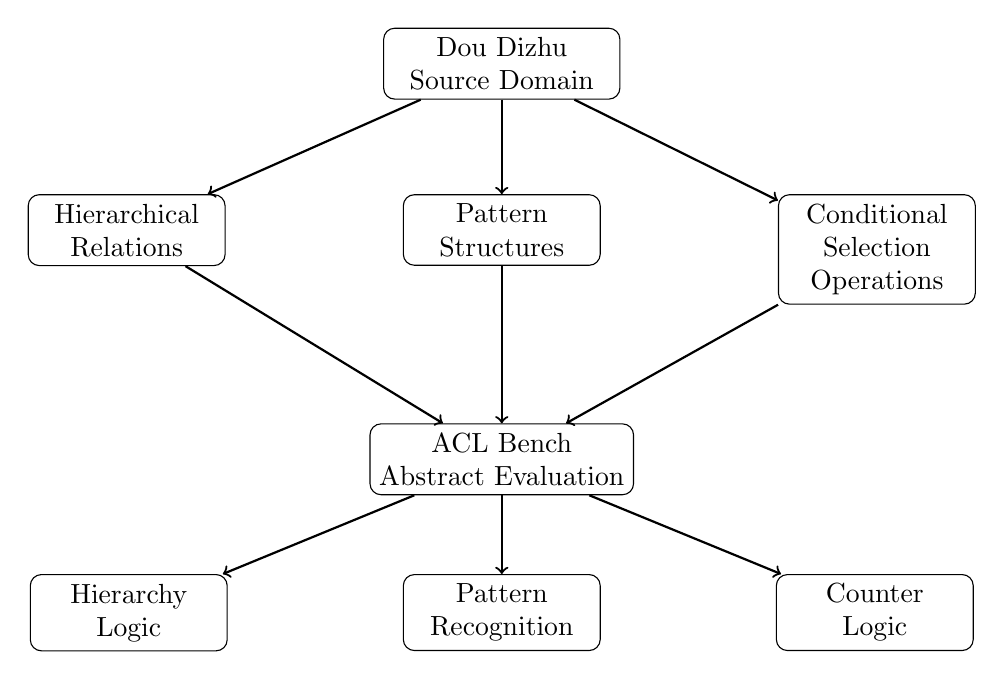
\begin{tikzpicture}[
node distance=1cm,
box/.style={
draw,
rounded corners,
align=center,
minimum width=3cm,
minimum height=0.8cm
},
smallbox/.style={
draw,
rounded corners,
align=center,
minimum width=2.5cm,
minimum height=0.7cm
},
arrow/.style={
->,
thick
}
]


% Source domain

\node (source) [box]
{Dou Dizhu\\
Source Domain};


% Abstract operations

\node (hier) [smallbox, below left=1.2cm and 2.0cm of source]
{
Hierarchical\\
Relations
};

\node (pattern) [smallbox, below=1.2cm of source]
{
Pattern\\
Structures
};

\node (counter) [smallbox, below right=1.2cm and 2.0cm of source]
{
Conditional\\
Selection\\
Operations
};


\draw[arrow] (source) -- (hier);
\draw[arrow] (source) -- (pattern);
\draw[arrow] (source) -- (counter);



% ACL Bench

\node (acl) [box, below=2cm of pattern]
{
ACL Bench\\
Abstract Evaluation
};


\node (logic1) [smallbox, below left=1cm and 1.8cm of acl]
{
Hierarchy\\
Logic
};


\node (logic2) [smallbox, below=1cm of acl]
{
Pattern\\
Recognition
};


\node (logic3) [smallbox, below right=1cm and 1.8cm of acl]
{
Counter\\
Logic
};


\draw[arrow] (hier) -- (acl);
\draw[arrow] (pattern) -- (acl);
\draw[arrow] (counter) -- (acl);


\draw[arrow] (acl) -- (logic1);
\draw[arrow] (acl) -- (logic2);
\draw[arrow] (acl) -- (logic3);


\end{tikzpicture}
\caption{
Construction of ACL Bench by abstracting Dou Dizhu decision operations into transferable reasoning categories.
The benchmark removes domain-specific surface forms while preserving underlying decision operations.
}
\label{fig:aclbench}
\end{figure}

We report overall and category-level accuracy for Base, DD-LoRA, and RC-LoRA. This three-way comparison separates the effect associated with ordinary Dou Dizhu mixed-data adaptation from the additional change observed in the constraint-enriched condition. Category-level results are retained because fine-tuning effects differ across reasoning types even when overall accuracy improves.

\subsection{Constraint-Sensitive Probe Evaluation}
\label{sec:constraint_probe_setup}

Constraint-induced relative preference shifts are evaluated with 60 controlled probes covering six decision scenarios. Each probe has a clean condition and a constrained condition in which an otherwise preferred action is explicitly prohibited. Evaluation uses seed 42, 16-bit floating-point (FP16) inference, scaled dot-product attention (SDPA), and batch size 1. We report mean BCDM across all 60 probes and per-scenario scores, using the metric defined in Section~\ref{sec:constraint_metric}; the six scenarios are reported in Table~\ref{tab:constraint_scenarios}. These probes are used to measure relative preference shifts under explicit prohibition rather than as an independent benchmark or a direct measure of generation compliance.

\subsection{Single-Head Causal Analysis}
\label{sec:causal_setup}

The complete attention-head scan is performed on Qwen2.5-7B, which has 28 Transformer layers and 28 attention heads per layer, for a total of 784 heads. Each head is ablated independently and the model is reevaluated on the same 60 constraint-sensitive probes. The scan is run for both Base and RC-LoRA, yielding 1,568 single-head intervention evaluations. For each head $(l,h)$, we compute $CE_{\mathrm{Base}}(l,h)$, $CE_{\mathrm{RC\text{-}LoRA}}(l,h)$, and $\Delta CE(l,h)$ as defined in Section~\ref{sec:head_ablation}. The resulting $28\times28$ map is used to analyze causal changes and rank heads for joint ablation.

\subsection{Top-k Joint-Ablation Evaluation}
\label{sec:topk_setup}

Joint ablation is evaluated at $k\in\{5,10,27\}$. For each $k$, we compare three conditions: \emph{Top-$k$}, consisting of the heads with the largest positive $\Delta CE$ values; \emph{Global Random}, sampled from all 784 heads; and \emph{Matched Random}, sampled to preserve the coarse layer-bin distribution of the corresponding Top-$k$ set across Layers 0--6, 7--13, 14--20, and 21--27. All joint-ablation runs use the same 60 probes, seed 42, FP16 inference, SDPA attention, and batch size 1. For each random-control condition, five independently sampled sets are generated with seeds 0--4, and their degradation scores are averaged.

The two random controls separate generic sensitivity to multi-head removal from effects attributable to broad depth-region concentration. Because the Matched Random condition is bin-matched rather than exact-layer matched, it does not eliminate all possible sensitivity differences among individual layers. A larger degradation under Top-$k$ than under both controls therefore supports additional functional relevance of the selected head identities beyond intervention size and coarse depth distribution. No additive assumption is made for joint interventions.

\subsection{Implementation Environment}
\label{sec:implementation_environment}

Fine-tuning and mechanistic experiments are conducted on an NVIDIA RTX A4500 GPU with 20~GB of memory. Gradient checkpointing is enabled during LoRA fine-tuning. Mechanistic evaluation uses mixed-precision inference where applicable and batch size 1 to support consistent head-level intervention.


% -----------------------------------------------------
% Caption color-key chips for result tables and figures.
% These commands are kept local to the Results section so no preamble edit is required.
% -----------------------------------------------------
\DeclareRobustCommand{\greenhl}[1]{%
  \begingroup\setlength{\fboxsep}{1.2pt}\colorbox{PositiveCell}{\strut #1}\endgroup}
\DeclareRobustCommand{\redhl}[1]{%
  \begingroup\setlength{\fboxsep}{1.2pt}\colorbox{NegativeCell}{\strut #1}\endgroup}
\DeclareRobustCommand{\neutralhl}[1]{%
  \begingroup\setlength{\fboxsep}{1.2pt}\colorbox{NeutralCell}{\strut #1}\endgroup}

\section{Results}
\label{sec:results}

This section reports the experimental results at three levels. We first evaluate cross-task transfer on ACL Bench for Base, DD-LoRA, and RC-LoRA across three open-weight checkpoints. We then examine constraint-induced relative preference shifts using controlled behavioral probes for Qwen2.5-7B. Finally, we analyze how rule-constrained fine-tuning changes the causal contribution of individual attention heads and validate the highest-ranked heads through joint Top-$k$ ablation against two random-control conditions.

\subsection{Task-Transfer Results}
\label{sec:task_transfer_results}

\subsubsection{Overall ACL Bench Performance}

Table~\ref{tab:acl_overall} and Figure~\ref{fig:acl_transfer} report overall ACL Bench accuracy for the three model states. DD-LoRA denotes ordinary mixed-data adaptation, whereas RC-LoRA denotes the constraint-enriched condition.

\begin{table}[H]
\centering
\caption{Overall ACL Bench accuracy for Base, DD-LoRA, and RC-LoRA. Values are percentages. $\Delta_{\mathrm{RC-DD}}$ is the RC-LoRA minus DD-LoRA difference in percentage points. \greenhl{Green-toned} highlighting marks positive RC-LoRA-over-DD-LoRA changes; unshaded black text is neutral.}
\label{tab:acl_overall}
\vspace{0.45em}
\begin{tabular}{lrrrr}
\toprule
\rowcolor{NeutralCell}
Model & Base & DD-LoRA & RC-LoRA & $\Delta_{\mathrm{RC-DD}}$ \\
\midrule
DeepSeek-R1-\allowbreak Distill-\allowbreak Llama-8B & 28.3 & 31.7 & 38.0 & \poscell{+6.3} \\
Qwen2.5-7B                  & 35.3 & 54.0 & 58.7 & \poscell{+4.7} \\
Llama3.1-8B                 & 45.0 & 42.3 & 46.7 & \poscell{+4.4} \\
\bottomrule
\end{tabular}
\end{table}

The ordinary DD-LoRA condition is strongly model-dependent. DeepSeek-R1-Distill-Llama-8B increases from 28.3\% to 31.7\%, and Qwen2.5-7B increases from 35.3\% to 54.0\%, whereas Llama3.1-8B decreases from 45.0\% to 42.3\%. Thus, ordinary mixed-data fine-tuning can produce substantial positive transfer for some checkpoints while inducing mild negative transfer for another.

RC-LoRA achieves 38.0\%, 58.7\%, and 46.7\% on DeepSeek-R1-Distill-Llama-8B, Qwen2.5-7B, and Llama3.1-8B, respectively. Relative to DD-LoRA, the corresponding overall changes are +6.3, +4.7, and +4.4 percentage points. Relative to Base, the RC-LoRA changes are +9.7, +23.4, and +1.7 percentage points. The consistent RC-LoRA-over-DD-LoRA direction across all three checkpoints indicates a more consistently positive transfer profile for the constraint-enriched regime than for the ordinary mixed-data regime. Figure~\ref{fig:acl_transfer} visualizes the three-way overall comparison and makes the DD-to-RC increment explicit for each checkpoint.

\begin{figure}[ht]
\centering
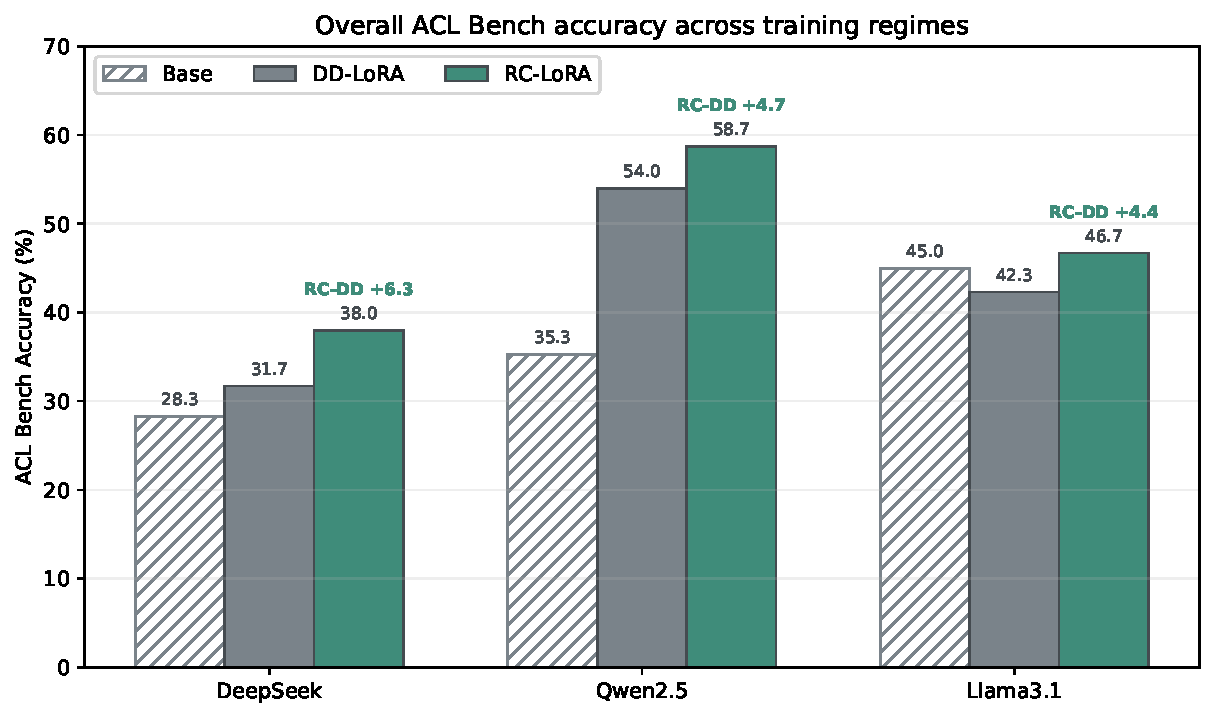
\includegraphics[width=0.86\linewidth]{figures/figure6_acl_transfer.pdf}
\caption{
Overall ACL Bench accuracy for Base, DD-LoRA, and RC-LoRA across the three evaluated checkpoints. The annotations above the RC-LoRA bars show the RC-LoRA minus DD-LoRA increment in percentage points. \greenhl{Green-toned} elements emphasize the focal RC-LoRA condition and its positive increment, whereas \neutralhl{gray/black or unfilled} elements denote neutral comparison states.
}
\label{fig:acl_transfer}
\end{figure}

\subsubsection{Category-Level Transfer}

Table~\ref{tab:acl_categories} reports category-level accuracy for Base, DD-LoRA, and RC-LoRA, while Figure~\ref{fig:acl_category_transfer} summarizes the corresponding Base-to-DD-LoRA and DD-LoRA-to-RC-LoRA changes.

\begin{table}[H]
\centering
\caption{Category-level ACL Bench accuracy for Base, DD-LoRA, and RC-LoRA. Values are percentages. \greenhl{Green-toned} RC-LoRA cells are higher than the corresponding DD-LoRA values; unshaded black entries are neutral.}
\label{tab:acl_categories}
\vspace{0.45em}
\begin{tabular}{llrrr}
\toprule
\rowcolor{NeutralCell}
Model & Setting & Counter & Hierarchy & Pattern \\
\midrule
DeepSeek & Base    & 24 & 35 & 26 \\
         & DD-LoRA & 28 & 30 & 37 \\
         & RC-LoRA & \poscell{37} & \poscell{40} & 37 \\
\midrule
Qwen2.5 & Base    & 34 & 36 & 36 \\
        & DD-LoRA & 39 & 60 & 63 \\
        & RC-LoRA & \poscell{46} & \poscell{65} & \poscell{65} \\
\midrule
Llama3.1 & Base    & 34 & 58 & 43 \\
         & DD-LoRA & 30 & 51 & 46 \\
         & RC-LoRA & 30 & \poscell{58} & \poscell{52} \\
\bottomrule
\end{tabular}
\end{table}

The DD-LoRA results already show selective transfer. For DeepSeek, Pattern Recognition improves from 26\% to 37\%, while Hierarchy Logic decreases from 35\% to 30\%. Qwen2.5 improves in all three categories, most strongly in Hierarchy Logic (36\% to 60\%) and Pattern Recognition (36\% to 63\%). Llama3.1 shows a smaller Pattern Recognition gain (43\% to 46\%) but decreases on Counter Logic and Hierarchy Logic.

Adding the constraint-enriched training regime produces a non-negative DD-LoRA-to-RC-LoRA change in every reported category. DeepSeek gains +9 points on Counter Logic and +10 on Hierarchy Logic while remaining unchanged on Pattern Recognition. Qwen2.5 gains +7, +5, and +2 points on Counter Logic, Hierarchy Logic, and Pattern Recognition, respectively. Llama3.1 remains unchanged on Counter Logic but gains +7 on Hierarchy Logic and +6 on Pattern Recognition.

These results support two distinctions. First, structural transfer is not introduced only by the constraint examples: ordinary DD-LoRA already produces large gains for some model--category pairs, particularly Qwen2.5 Hierarchy Logic and Pattern Recognition. Second, the constraint-enriched RC-LoRA condition is associated with a consistent positive overall increment relative to DD-LoRA and with non-negative category-level changes across the three evaluated checkpoints. The effect is therefore better characterized as selective and model-dependent transfer with an additional cross-checkpoint consistency in the RC-LoRA-over-DD-LoRA direction, rather than as a uniform increase in general reasoning ability. Figure~\ref{fig:acl_category_transfer} separates the two transition stages visually: the left panel shows Base $\rightarrow$ DD-LoRA changes, and the right panel shows the additional DD-LoRA $\rightarrow$ RC-LoRA changes.

\begin{figure}[ht]
\centering
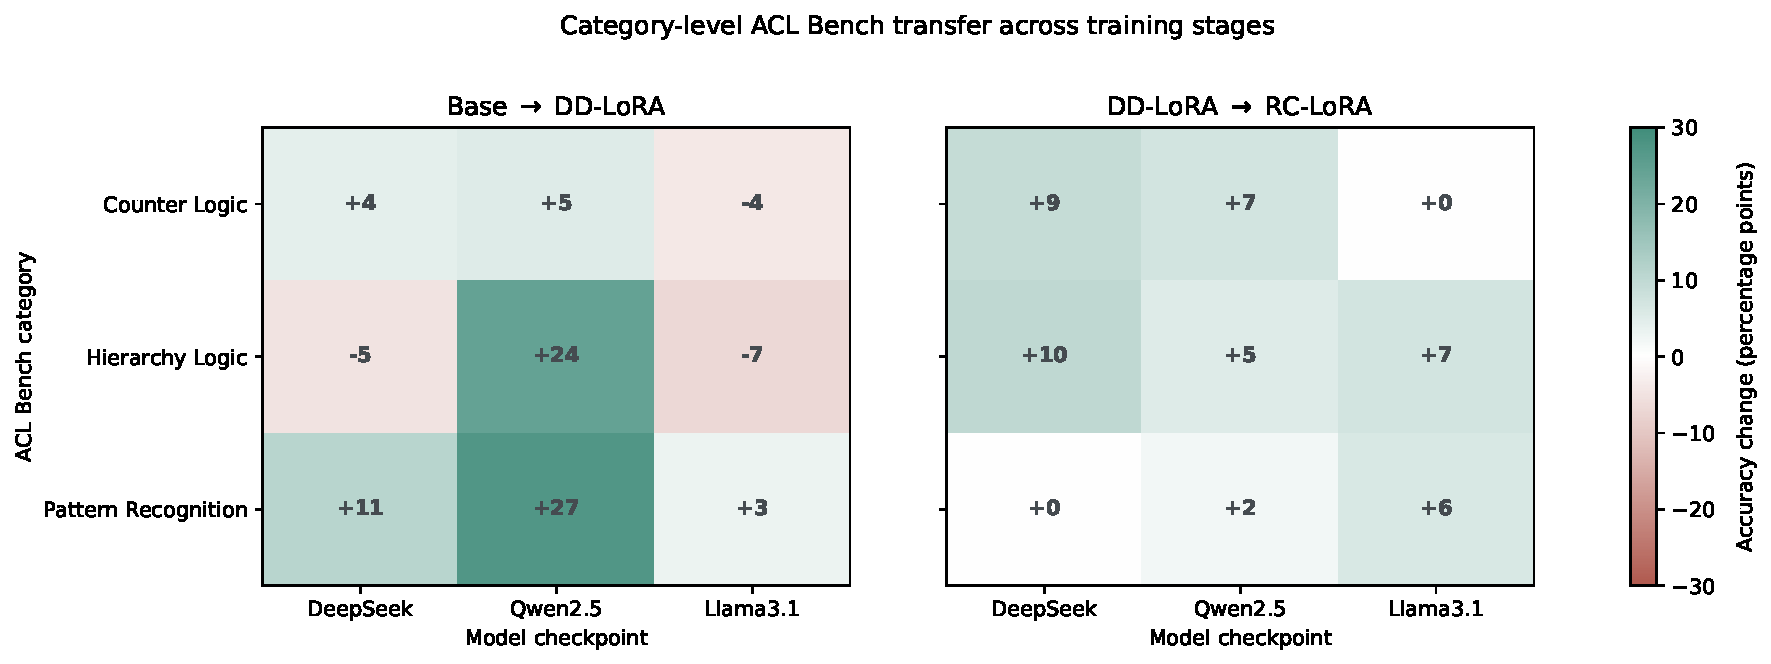
\includegraphics[width=0.96\linewidth]{figures/figure7_acl_category_transfer.pdf}
\caption{
Category-level ACL Bench transfer across training stages. Left: Base-to-DD-LoRA accuracy changes. Right: DD-LoRA-to-RC-LoRA accuracy changes. \greenhl{Green-toned} cells indicate positive accuracy changes, \redhl{red-toned} cells indicate negative changes, and \neutralhl{neutral-toned} cells indicate values near zero.
}
\label{fig:acl_category_transfer}
\end{figure}

\subsection{Constraint-Sensitive Preference-Shift Results}
\label{sec:constraint_behavior_results}

ACL Bench evaluates transfer outside the source domain, but it does not directly measure whether the fine-tuned model has learned to revise its decision preference when an additional rule prohibits an otherwise preferred action. We therefore evaluate Qwen2.5-7B Base and RC-LoRA on the 60 controlled constraint-sensitive probes using BCDM.

\subsubsection{Overall Relative-Preference Shift}

Table~\ref{tab:constraint_overall} summarizes the overall preference-shift scores.

\begin{table}[t]
\centering
\caption{BCDM on the 60 constraint-sensitive probes. Values are reported as mean $\pm$ standard deviation. \greenhl{Green-toned} highlighting marks the higher BCDM relative-preference-shift score compared with Base; unshaded black entries are neutral.}
\label{tab:constraint_overall}
\vspace{0.45em}
\begin{tabular}{lc}
\toprule
\rowcolor{NeutralCell}
Model & BCDM \\
\midrule
Qwen2.5-7B Base & $1.391 \pm 1.379$ \\
Qwen2.5-7B RC-LoRA & \poscell{$4.371 \pm 0.766$} \\
\bottomrule
\end{tabular}
\end{table}

Mean BCDM increases from $1.391 \pm 1.379$ for the Base model to $4.371 \pm 0.766$ for RC-LoRA, a gain of approximately 2.981 points. Because BCDM measures the change in the relative log-probability margin between the forbidden action and the strongest legal alternative, the increase indicates a larger constraint-induced relative preference shift in RC-LoRA. The relatively large standard deviation of the Base model is consistent with the heterogeneous scenario-level behavior reported below: several scenarios produce small mean shifts, whereas \path{straight_34567} already produces a much larger Base response. The aggregate Base score therefore combines probes with substantially different levels of constraint sensitivity rather than reflecting a uniformly distributed response, while RC-LoRA shows a smaller standard deviation and a more consistent BCDM response across the evaluated probes. Importantly, BCDM should not be interpreted as final-action compliance: a positive BCDM can coexist with the forbidden action remaining the highest-probability output, so the metric does not by itself indicate that a legal alternative becomes the generated action.

\subsubsection{Scenario-Level Results}

The 60 probes are divided equally across six controlled scenarios, with 10 probes per scenario. Table~\ref{tab:constraint_scenarios} reports the corresponding mean scores.

\begin{table}[t]
\centering
\caption{Scenario-level BCDM for Qwen2.5-7B. Each scenario contains 10 probes. \greenhl{Green-toned} $\Delta$ values indicate larger BCDM after fine-tuning, \redhl{red-toned} values indicate a decline, and unshaded black entries are neutral references.}
\label{tab:constraint_scenarios}
\vspace{0.45em}
\begin{tabular}{lrrr}
\toprule
\rowcolor{NeutralCell}
Scenario & Base & RC-LoRA & $\Delta$ \\
\midrule
\path{bomb_9999}              & 1.898 & 4.180 & \poscell{+2.282} \\
\path{pair_88}                & 0.309 & 5.284 & \poscell{+4.975} \\
\path{real_pair_QQ_landlord}& 0.155 & 4.107 & \poscell{+3.952} \\
\path{rocket_BR}              & 1.115 & 5.427 & \poscell{+4.312} \\
\path{single_A_follow}       & 0.700 & 3.252 & \poscell{+2.552} \\
\path{straight_34567}         & 4.168 & 3.977 & \negcell{-0.191} \\
\bottomrule
\end{tabular}
\end{table}

RC-LoRA achieves a higher constraint-sensitive score in five of the six scenarios, with the largest gains of 4.975 for \path{pair_88}, 4.312 for \path{rocket_BR}, and 3.952 for \path{real_pair_QQ_landlord}. The \path{straight_34567} scenario differs from the others: the Base model already exhibits a relatively high score of 4.168, while the RC-LoRA score is slightly lower at 3.977. The fine-tuning effect is therefore not uniformly positive across every individual scenario. Nevertheless, the overall mean increases substantially, and five of the six scenario-level comparisons show a larger BCDM for RC-LoRA. These results support a cross-scenario increase in the measured constraint-induced relative preference shift while also indicating that the magnitude of the effect depends on the underlying decision structure.

\begin{figure}[ht]
\centering
\resizebox{0.98\linewidth}{!}{%
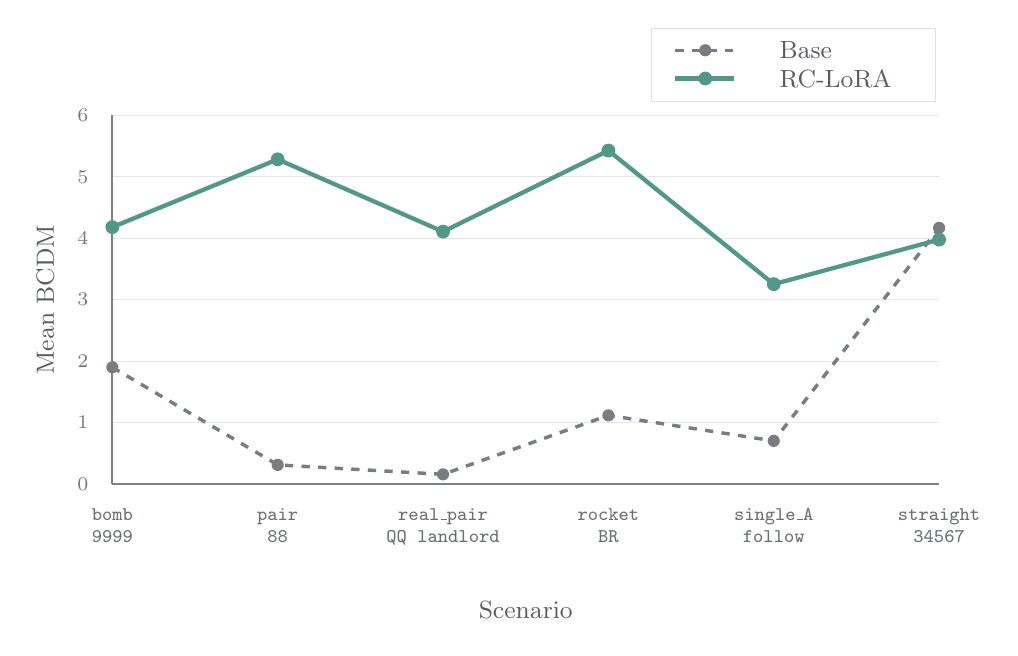
\begin{tikzpicture}[x=1cm,y=0.78cm]

% Plot area
\def\xmax{10.5}
\def\ymax{6}

% Horizontal grid and y-axis ticks
\foreach \y in {0,1,2,3,4,5,6} {
    \draw[draw=Ink!14,line width=0.35pt] (0,\y) -- (\xmax,\y);
    \node[font=\scriptsize,anchor=east,text=Ink!75] at (-0.18,\y) {\y};
}

% Axes
\draw[draw=Ink!70,line width=0.7pt] (0,0) -- (\xmax,0);
\draw[draw=Ink!70,line width=0.7pt] (0,0) -- (0,\ymax);

% Axis labels
\node[font=\small,rotate=90,text=Ink!90] at (-0.85,3) {Mean BCDM};
\node[font=\small,text=Ink!90] at (5.25,-2.05) {Scenario};

% X-axis scenario labels
\node[font=\scriptsize\ttfamily,align=center,anchor=north,text=Ink!80]
    at (0, -0.24) {bomb\\9999};
\node[font=\scriptsize\ttfamily,align=center,anchor=north,text=Ink!80]
    at (2.1, -0.24) {pair\\88};
\node[font=\scriptsize\ttfamily,align=center,anchor=north,text=Ink!80]
    at (4.2, -0.24) {real\_pair\\QQ landlord};
\node[font=\scriptsize\ttfamily,align=center,anchor=north,text=Ink!80]
    at (6.3, -0.24) {rocket\\BR};
\node[font=\scriptsize\ttfamily,align=center,anchor=north,text=Ink!80]
    at (8.4, -0.24) {single\_A\\follow};
\node[font=\scriptsize\ttfamily,align=center,anchor=north,text=Ink!80]
    at (10.5, -0.24) {straight\\34567};

% Base: dashed line for grayscale readability
\draw[draw=Ink!72,line width=1.25pt,dashed]
    (0,1.898) --
    (2.1,0.309) --
    (4.2,0.155) --
    (6.3,1.115) --
    (8.4,0.700) --
    (10.5,4.168);

% RC-LoRA: solid line
\draw[draw=Positive!90,line width=1.55pt]
    (0,4.180) --
    (2.1,5.284) --
    (4.2,4.107) --
    (6.3,5.427) --
    (8.4,3.252) --
    (10.5,3.977);

% Data-point markers
\foreach \x/\y in {0/1.898,2.1/0.309,4.2/0.155,6.3/1.115,8.4/0.700,10.5/4.168} {
    \fill[Ink!72] (\x,\y) circle (2.2pt);
}
\foreach \x/\y in {0/4.180,2.1/5.284,4.2/4.107,6.3/5.427,8.4/3.252,10.5/3.977} {
    \fill[Positive!90] (\x,\y) circle (2.5pt);
}

% Legend placed above the plotting area so it never covers the data lines
\draw[draw=Ink!18,fill=white,line width=0.35pt] (6.85,6.22) rectangle (10.45,7.42);

\draw[draw=Ink!72,line width=1.25pt,dashed] (7.15,7.06) -- (7.90,7.06);
\fill[Ink!72] (7.53,7.06) circle (2.2pt);
\node[font=\small,anchor=west,text=Ink!90] at (8.35,7.06) {Base};

\draw[draw=Positive!90,line width=1.55pt] (7.15,6.60) -- (7.90,6.60);
\fill[Positive!90] (7.53,6.60) circle (2.5pt);
\node[font=\small,anchor=west,text=Ink!90] at (8.35,6.60) {RC-LoRA};

\end{tikzpicture}%
}

\caption{
Scenario-level BCDM for Qwen2.5-7B Base and RC-LoRA across six constraint-sensitive scenarios. Each point is the mean over 10 probes. The \greenhl{green-toned} line denotes the focal RC-LoRA condition, while the \neutralhl{black/gray} line is the neutral Base reference; scenario-wise improvement or decline is determined by their relative heights.
}
\label{fig:preference_shift}
\end{figure}

\subsubsection{Preference--Generation Gap}

The larger probability-level relative shift does not translate into better greedy-decoding compliance. Under direct generation, the Base model selects the forbidden action in 40 of 60 probes (66.7\%) and a legal action in the remaining 20 probes; 10 of these legal outputs match the designated allowed action and 10 are other legal alternatives. RC-LoRA selects the forbidden action in all 60 probes. Thus, the legal-action rate decreases from 33.3\% for Base to 0\% for RC-LoRA.

This diagnostic establishes a clear separation between the BCDM-based relative preference shift and executable compliance. The current results do not show improved rule-compliant generation after RC-LoRA; instead, they show that the constraint produces a larger change in the relative legal-versus-forbidden margin even though the forbidden action still wins under greedy decoding. The mechanistic analyses below therefore concern the probability-level effect measured by BCDM, not final-action compliance.


\subsection{Attention-Head Causal Results}
\label{sec:head_causal_results}

RC-LoRA shows a substantially larger BCDM than the Base model. We next examine whether this Base-to-RC difference is accompanied by changes in the functional importance of individual attention heads, focusing the causal analysis on Qwen2.5-7B.

\subsubsection{Exploratory Attention-Based Screening}

Before performing the complete intervention scan, we explored whether constraint-related attention heads could be identified through a three-stage attention-based screening procedure consisting of targeting, correlation, and counterfactual filtering. For the Base model, the screening sequence was $784\rightarrow157\rightarrow22\rightarrow14$ candidate heads. The standard RC-LoRA sequence was $784\rightarrow157\rightarrow0\rightarrow0$. Under a relaxed RC-LoRA setting using 100 samples, the targeting stage retained 235 heads, but none survived the subsequent correlation stage ($784\rightarrow235\rightarrow0\rightarrow0$). These results indicate that simple attention--behavior correlation does not provide a stable basis for identifying constraint-relevant components after fine-tuning; rather than treating the absence of correlated heads as evidence that the model lacks localized functional dependence, we therefore proceed to direct causal intervention.

\subsubsection{Complete Single-Head Causal Scan}

Qwen2.5-7B contains 28 Transformer layers with 28 attention heads per layer, yielding 784 heads in total. Each head is independently ablated in both the Base and RC-LoRA models, producing 1,568 single-head interventions. For every intervention, we compute the causal contribution and the Base-to-RC-LoRA change $\Delta CE(l,h)$ defined in Eq.~\ref{eq:delta_ce}. The resulting distribution is highly heterogeneous: most heads show relatively small causal changes, while a much smaller subset exhibits substantially larger positive $\Delta CE$ values.

\begin{figure}[t]
\centering
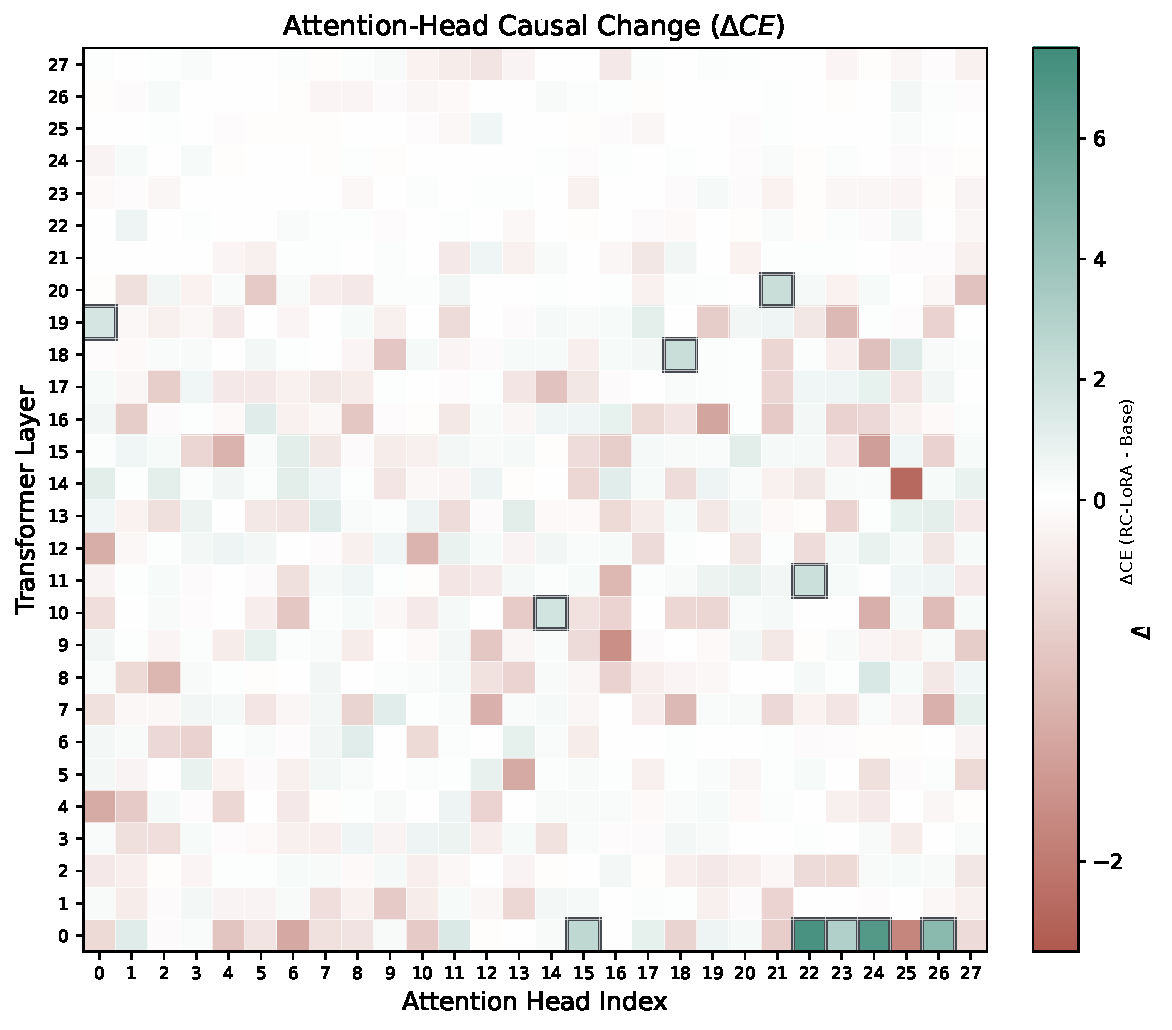
\includegraphics[width=0.78\linewidth]{figures/figure_attention_head_heatmap.pdf}
\caption{
Attention-head heatmap of Base-to-RC-LoRA causal change $\Delta CE$ for Qwen2.5-7B.
Rows correspond to Transformer layers and columns correspond to attention-head indices.
\greenhl{Green-toned} hues indicate $\Delta CE>0$, \redhl{red-toned} hues indicate $\Delta CE<0$, and near-neutral tones indicate values close to zero. \neutralhl{Black} outlines are neutral markers that identify the ten heads with the largest positive causal changes.
The distribution shows sparse and heterogeneous redistribution of causal dependence across attention heads.
}
\label{fig:attention_heatmap}
\end{figure}

Negative values are also observed, indicating that some heads become less supportive of the measured behavior after fine-tuning or that their removal improves the preference-shift score. Together, the positive and negative changes show that causal dependence is redistributed non-uniformly rather than uniformly strengthened across the attention system. Figure~\ref{fig:layerwise_delta_ce} summarizes the positive component of this redistribution across Transformer layers.

\begin{figure}[!tbp]

\centering

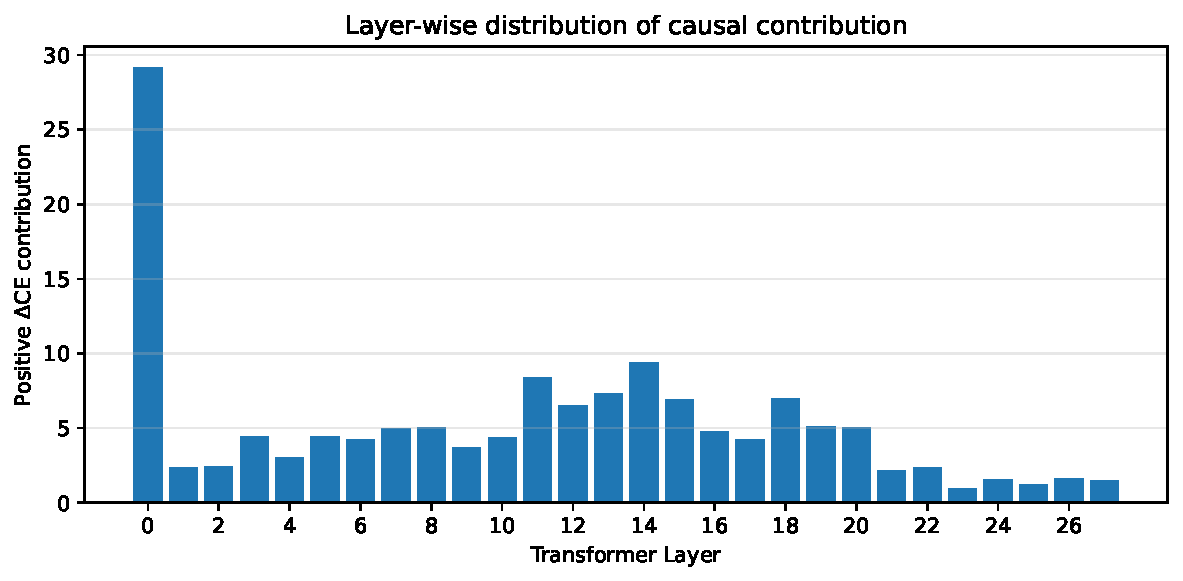
\includegraphics[
width=0.85\linewidth
]{figures/figure8_layerwise_delta_ce.pdf}

\caption{
Layer-wise distribution of positive causal contribution measured by $\Delta CE$ across Qwen2.5-7B attention heads. The \greenhl{green-toned} bars represent positive causal-change contributions, while black/gray axes and grid elements are neutral visual references. The distribution shows non-uniform changes in causal contribution across Transformer layers after fine-tuning.
}

\label{fig:layerwise_delta_ce}

\end{figure}

The layer-wise pattern remains non-uniform, and Table~\ref{tab:top_heads} reports the ten heads with the largest positive $\Delta CE$ values.

\begin{table}[t]
\centering
\caption{Top ten Qwen2.5-7B attention heads ranked by Base-to-RC-LoRA causal change $\Delta CE$. All listed heads exhibit positive $\Delta CE$, indicating higher causal contribution in RC-LoRA than in Base under the present metric.}
\label{tab:top_heads}
\vspace{0.45em}
\begin{tabular}{rrr}
\toprule
\rowcolor{NeutralCell}
Rank & Attention Head & $\Delta CE$ \\
\midrule
1  & L0-H22  & 7.062 \\
2  & L0-H24  & 6.671 \\
3  & L0-H26  & 4.552 \\
4  & L0-H23  & 2.996 \\
5  & L0-H15  & 2.486 \\
6  & L20-H21 & 2.101 \\
7  & L18-H18 & 2.055 \\
8  & L11-H22 & 2.046 \\
9  & L10-H14 & 1.746 \\
10 & L19-H0  & 1.595 \\
\bottomrule
\end{tabular}
\end{table}

Several of the strongest causal changes are concentrated in Layer 0: five of the ten highest-ranked heads are located in the first Transformer layer. However, positive $\Delta CE$ values are not restricted to the earliest layer, with additional top-ranked heads appearing in Layers 10, 11, 18, 19, and 20. The pattern therefore combines strong early-layer concentration with additional high-impact components distributed across intermediate layers, rather than indicating a mechanism confined to a single network depth.

\subsubsection{Representative Head: L0-H22}

L0-H22 provides the clearest example of causal amplification after fine-tuning. In the Base model, ablating this head reduces the preference-shift score from 1.390711 to 0.751787, giving $CE_{\mathrm{Base}}=0.638924$. In RC-LoRA, the same ablation changes the score from 4.371395 to $-3.329531$, giving $CE_{\mathrm{RC\text{-}LoRA}}=7.700926$. The resulting Base-to-RC-LoRA change is therefore $\Delta CE=7.062002$. L0-H22 is thus already positively involved in the measured behavior before fine-tuning, but its causal contribution becomes much larger afterward. This pattern is consistent with selective amplification or functional reconfiguration of an existing component rather than the appearance of an entirely new attention-head function.

\subsubsection{Causal Heterogeneity Across Heads}

The complete scan reveals several qualitatively different patterns of causal change. Some heads satisfy $CE_{\mathrm{RC\text{-}LoRA}}\gg CE_{\mathrm{Base}}>0$, indicating strong amplification of an already positive Base-model contribution, while others have weak Base contributions but become substantially positive after fine-tuning. Many heads remain near $\Delta CE\approx0$, whereas a smaller subset has $\Delta CE<0$, showing that fine-tuning can also reduce the measured contribution of individual components. Together, these results support a sparse and non-uniform redistribution of causal dependence rather than uniform strengthening of attention heads across the network, and they help explain why attention-based correlation alone is insufficient for identifying the relevant components: strong causal importance after fine-tuning does not necessarily correspond to a simple observable attention--behavior correlation.

\subsubsection{Top-k Joint-Ablation Validation}

Single-head causal effects identify components whose individual importance changes after fine-tuning, but they do not establish whether the highest-ranked heads form a collectively important functional subset. We therefore jointly ablate the Top-$k$ heads ranked by $\Delta CE$ for $k\in\{5,10,27\}$ and compare the resulting behavioral degradation against Global Random and Matched Random controls, each averaged over five independently sampled control sets; the comparison is summarized in Figure~\ref{fig:topk_validation}.

\begin{figure}[ht]
\centering

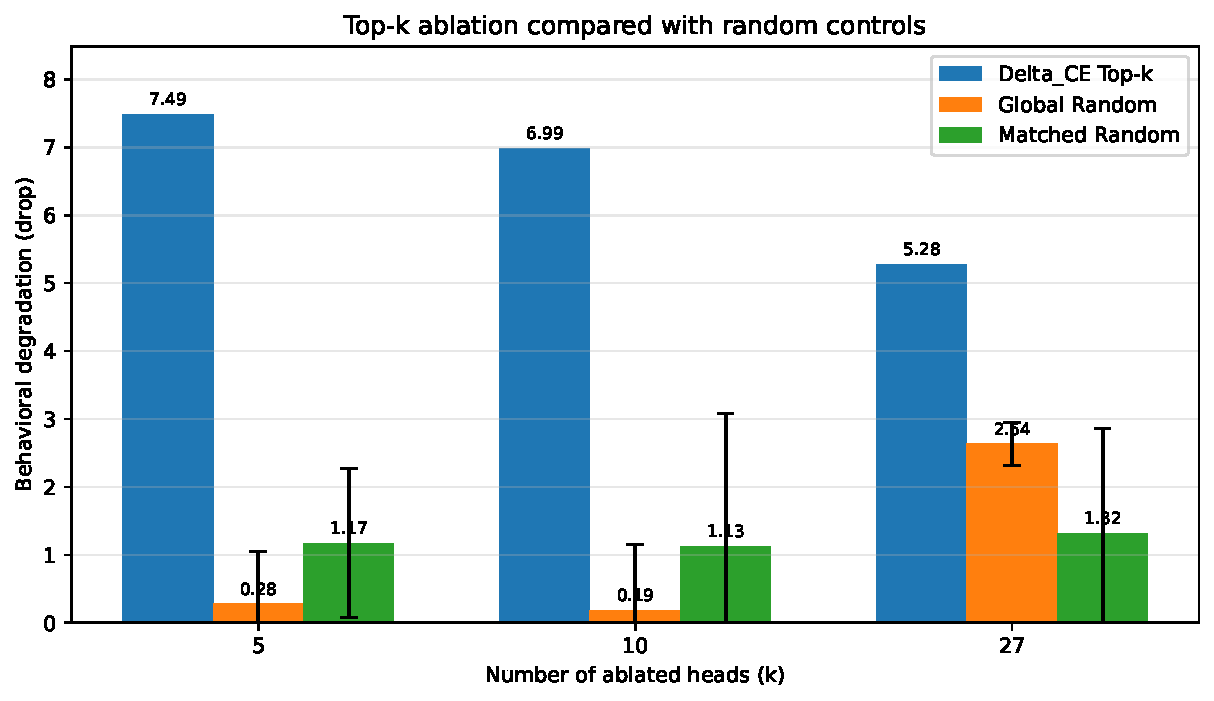
\includegraphics[width=0.65\linewidth]{figures/figure4b_random_controls.pdf}


\vspace{0.2cm}


\begin{minipage}{0.7\linewidth}
\centering
\scriptsize

\begin{tabular}{rrrr}
\toprule
\rowcolor{NeutralCell}
$k$ & Top-$k$ & Global Random & Matched Random \\
\midrule
5  & \poscell{7.489} & \neutralcell{0.281} & \neutralcell{1.173} \\
10 & \poscell{6.987} & \neutralcell{0.186} & \neutralcell{1.130} \\
27 & \poscell{5.281} & \neutralcell{2.638} & \neutralcell{1.320} \\
\bottomrule
\end{tabular}

\end{minipage}


\caption{
Joint-ablation validation of attention heads selected by fine-tuning-induced causal change.
Here, $\Delta CE=CE_{\mathrm{RC\text{-}LoRA}}-CE_{\mathrm{Base}}$ denotes the Base-to-RC-LoRA change in head-level causal effect, and the Top-$k$ set contains the $k$ heads with the largest positive $\Delta CE$ values.
Global Random and Matched Random are equal-size controls; Matched Random preserves the Top-$k$ distribution across four coarse layer bins rather than matching exact layers. Error bars indicate standard deviation across five random-control runs. \greenhl{Green-toned} bars/cells denote the focal $\Delta CE$-selected Top-$k$ intervention, whereas \neutralhl{gray/black or unfilled} bars/cells denote neutral random-control comparisons.
}

\label{fig:topk_validation}

\end{figure}


Across all three intervention sizes, Top-$k$ ablation causes greater behavioral degradation than either random control. At $k=5$, removing the five highest-ranked heads produces a drop of 7.489, compared with 0.281 under Global Random and 1.173 under Matched Random. At $k=10$, the Top-$k$ drop remains large at 6.987, whereas Global Random and Matched Random produce drops of only 0.186 and 1.130, respectively. At $k=27$, Top-$k$ ablation produces a drop of 5.281; although the Global Random effect becomes larger at this intervention size, reaching 2.638, it remains substantially below the Top-$k$ effect, while the corresponding Matched Random drop is 1.320. Within the evaluated 60-probe set, these results support the view that the $\Delta CE$ ranking identifies a functionally distinctive subset of attention heads relative to the two sampled random controls.

The Global Random comparison shows that the result cannot be explained simply by removing the same number of arbitrary attention heads. The Matched Random comparison provides a stricter control than Global Random by preserving the coarse layer-bin distribution of the Top-$k$ set. The persistence of a larger Top-$k$ effect under this control indicates that broad depth-region concentration alone is insufficient to reproduce the observed degradation in these runs. Because matching is performed at the bin level rather than at the exact-layer level, residual sensitivity differences among individual layers remain a possible confound. In addition, the same 60 probes are used to rank heads and to evaluate the joint Top-$k$ interventions, so this experiment is an in-sample functional validation rather than a held-out test of head-set generalization.

\FloatBarrier

\subsubsection{Non-Monotonic Joint-Ablation Effects}

An important feature of the Top-$k$ results is that behavioral degradation does not increase monotonically with $k$: the Top-$k$ drops are 7.489, 6.987, and 5.281 for $k=5$, 10, and 27, respectively. Removing additional high-ranked heads therefore does not produce progressively larger degradation. This pattern is consistent with the non-additive formulation in Eq.~\ref{eq:nonadditive_heads} and may reflect redundancy, compensation, inhibitory interactions, or other nonlinear dependencies among attention heads. The present experiment does not distinguish among these possibilities; nevertheless, it shows that a relatively small set of highly ranked heads can have a particularly strong joint effect and that extending the intervention to a larger set changes the functional interaction among the remaining components.

Overall, the causal analyses show a sparse and heterogeneous redistribution of head-level dependence after fine-tuning. The highest-ranked heads form a functionally distinctive subset under joint ablation, but these interventions directly explain BCDM-based preference adaptation rather than the mechanism of ACL Bench transfer.




\section{Discussion}
\label{sec:discussion}

The results indicate selective rather than uniform changes across training regimes. DD-LoRA already alters ACL Bench performance substantially, but the direction and magnitude depend on the underlying checkpoint. RC-LoRA is higher than DD-LoRA in overall ACL Bench accuracy for all three evaluated checkpoints, while the category-level effects remain heterogeneous. For Qwen2.5-7B, RC-LoRA also exhibits a larger BCDM than Base and a different pattern of causal dependence across a limited subset of attention heads. These effects are related, but they should not be collapsed into a single claim of general capability improvement.

\subsection{Selective and Model-Dependent Transfer}
\label{sec:discussion_transfer}

The three-way ACL Bench comparison separates two effects that were conflated in a Base-versus-RC-LoRA analysis. First, ordinary structured-task adaptation already produces substantial transfer in some settings. DeepSeek-R1-Distill-Llama-8B increases from 28.3\% to 31.7\% overall under DD-LoRA, and Qwen2.5-7B increases from 35.3\% to 54.0\%, whereas Llama3.1-8B decreases from 45.0\% to 42.3\%. Ordinary Dou Dizhu adaptation therefore does not provide a uniformly beneficial transfer signal. Second, RC-LoRA is higher than DD-LoRA in overall ACL Bench accuracy for all three checkpoints: 31.7\% to 38.0\% for DeepSeek, 54.0\% to 58.7\% for Qwen2.5, and 42.3\% to 46.7\% for Llama3.1. The category-level changes from DD-LoRA to RC-LoRA are also non-negative in all nine model--category comparisons, although their magnitudes differ: DeepSeek gains primarily on Counter and Hierarchy Logic, Qwen2.5 improves across all three categories, and Llama3.1 gains on Hierarchy Logic and Pattern Recognition while remaining unchanged on Counter Logic.

This pattern argues against interpreting fine-tuning as a task-independent increase in reasoning ability. A more plausible interpretation is that ordinary structured-task training strengthens some reusable operations but can also induce capability trade-offs, whereas the constraint-enriched regime is associated with a more consistently positive transfer profile across the evaluated checkpoints. We therefore describe the observed effect as \emph{selective structural transfer with constraint-associated cross-checkpoint consistency}. The relevant unit of transfer is not necessarily the source task as a whole, but operations such as ordered comparison, pattern processing, and conditional action selection.

\subsection{Constraint-Induced Relative Preference Shift and the Generation Gap}
\label{sec:discussion_preference}

The constraint-sensitive probes clarify what the current BCDM result does and does not establish. BCDM measures how an explicit prohibition changes the relative log-probability margin between the forbidden action and the strongest legal alternative. The substantially larger mean BCDM for RC-LoRA therefore indicates a larger constraint-induced relative preference shift than in Base, but it should not be interpreted as direct evidence that probability mass is successfully redirected enough to change the model's final decision. The direct-generation diagnostic makes this distinction explicit. Base produces a legal action in 20 of 60 probes, whereas RC-LoRA produces the forbidden action in all 60. The present evidence therefore does not support a claim that RC-LoRA improves executable constraint following under greedy decoding. Instead, it shows a probability-level change in the legal-versus-forbidden margin that remains insufficient to move the generated output across the decision boundary. This preference--generation gap is itself informative: a model can become more responsive to a constraint in relative candidate scores while becoming no more, or even less, compliant at the final-action level.

The constraint-injected examples differ from ordinary state--action supervision because the appropriate supervised target can depend on an additional rule: the same underlying state may require a different target once a preferred option becomes invalid. The paired probes therefore provide a direct behavioral view of how the RC-LoRA model responds when the admissible action space is explicitly changed.

\subsection{Sparse and Non-Additive Causal Reorganization}
\label{sec:discussion_reconfiguration}

The complete Qwen2.5-7B head scan reveals changes in causal dependence unevenly across attention heads. Most heads exhibit relatively small Base-to-RC-LoRA changes, whereas a much smaller subset shows large positive $\Delta CE$ values and some heads show negative changes. This distribution is inconsistent with uniform strengthening of the attention system and instead supports a selective reorganization of functional dependence. L0-H22 provides a representative example. The head contributes positively to the measured behavior in the Base model and becomes substantially more important after fine-tuning. This is consistent with prior findings that fine-tuning can amplify mechanisms already present in a pretrained model rather than necessarily constructing entirely new computational structures \cite{prakash2024finetuning}. The present evidence supports this interpretation for some heads, but not as a universal account of every causal change.

The Top-$k$ experiments provide a stronger test than single-head ranking alone. Joint ablation of the highest-ranked heads produces greater degradation than both global-random and layer-bin-matched random controls, showing that the selected head set carries information beyond intervention size and broad depth-region placement. At the same time, degradation is non-monotonic as $k$ increases. Individual head effects therefore cannot be treated as additive; redundancy, compensation, inhibitory interactions, or larger network-state changes may contribute to the joint-ablation pattern.

The exploratory attention-based screening also differs from the causal results. More generally, prior work cautions against treating attention-based signals as faithful explanations of model behavior \cite{jain2019attention}. The absence of RC-LoRA heads surviving the correlation-based screening therefore does not imply an absence of functionally important heads, because causal ablation identifies several with large behavioral effects. Attention correlation and causal contribution should be treated as distinct quantities.

Several high-$\Delta CE$ heads occur in early layers, but the strongest effects are not confined there. High-impact heads also appear at intermediate depths, and the layer-bin-matched controls show that the Top-$k$ effect is not reproduced by matching only the broad depth profile. However, because exact layers are not matched, generic sensitivity differences among individual layers cannot be fully excluded. The causal redistribution is therefore better characterized as sparse and distributed across depth, with this remaining control limitation made explicit.

\subsection{Scope, Limitations, and Causal Boundary}
\label{sec:limitations}

The behavioral and mechanistic results should be interpreted at different levels. ACL Bench provides evidence of selective cross-task transfer. The constraint probes measure a larger constraint-induced relative preference shift for RC-LoRA than for Base, while the direct-generation diagnostic shows that this does not amount to improved executable compliance. The attention-head interventions establish causal support for the BCDM-based preference shift within the Base-to-RC comparison, but the current experiments do not directly show that the same heads are responsible for ACL Bench gains. This distinction is important because the mechanistic analysis is evaluated with BCDM rather than ACL Bench. A direct causal bridge would require evaluating ACL Bench under the same Top-$k$ and appropriately matched interventions. Stronger ACL degradation under Top-$k$ ablation would support a shared internal basis between constraint adaptation and transfer; stable ACL performance would instead suggest partially distinct mechanisms.

Several additional limitations remain. Dou Dizhu is the only source domain, and ACL Bench is intentionally constructed around structurally related operations, so broader generalization requires additional source domains and independent benchmarks. Complete causal analysis is currently available only for Qwen2.5-7B, and the present attention-head interventions characterize a selected set of functionally important components rather than a complete circuit. The Top-$k$ experiment is also an in-sample validation because the same 60 probes are used both to rank heads by $\Delta CE$ and to evaluate joint ablation. In addition, each random-control mean is based on five sampled head sets, so the controls should be interpreted descriptively rather than as a full randomization distribution. Top-$k$ ablation therefore identifies a functionally important subset for the present probe set, not a complete circuit or a held-out mechanistic signature.

The most informative extensions are held-out or cross-validated Top-$k$ validation, direct ACL Bench ablation with Top-$k$ and corresponding controls, causal replication on additional checkpoints, and evaluation on additional source domains and independent benchmarks. Interaction analysis among the highest-ranked heads would also help distinguish redundancy, compensation, and other sources of the observed non-monotonic joint effects.




\section{Conclusion}
\label{sec:conclusion}

This study examines whether structured fine-tuning on Dou Dizhu transfers beyond the source domain, how rule-constrained supervision alters model preferences under explicit prohibitions, and how these behavioral changes are reflected in attention-head-level causal dependence. Across DeepSeek-R1-Distill-Llama-8B, Qwen2.5-7B, and Llama3.1-8B, DD-LoRA exhibits strongly model-dependent transfer on ACL Bench, whereas RC-LoRA achieves higher overall accuracy than DD-LoRA in each case, with category-level effects remaining selective rather than uniform. For Qwen2.5-7B, RC-LoRA produces a substantially larger BCDM than Base, indicating a larger constraint-induced relative preference shift; however, this probability-level change does not translate into improved greedy-decoding compliance, as RC-LoRA selects the prohibited action in all 60 probes. Ablation of individual attention heads further reveals a sparse and heterogeneous redistribution of causal dependence, with a small subset of heads contributing disproportionately to the measured preference shift. Top-$k$ joint ablation produces greater degradation than both global-random and layer-bin-matched random controls, while the non-monotonic effects indicate that head contributions are not simply additive. Overall, these findings support selective cross-task transfer and selective causal reorganization rather than uniform capability gain. They also show that task-transfer performance, constraint-induced preference reallocation, executable rule compliance, and internal causal dependence are distinct outcomes of fine-tuning and should be evaluated separately.


\bibliographystyle{elsarticle-num}
\bibliography{references}

\end{document}



